\documentclass[apjl,twocolumn]{emulateapj}
\usepackage{graphicx}
\usepackage[varg]{txfonts}
%\usepackage[pagebackref,breaklinks,colorlinks,citecolor=blue]{hyperref}        
\usepackage[%draft, pagebackref,
colorlinks,citecolor=blue,linkcolor=blue,urlcolor=blue]{hyperref}
%\renewcommand*{\backref}[1]{[#1]}  % gives neat back references in the pdf
\usepackage{aas_macros}
%\usepackage{amsmath} % clashes with emulateapjj for some reaons
\usepackage[usenames,dvipsnames]{xcolor}
\usepackage{comment}
\usepackage{multirow}
%\usepackage{chngpage}
%\usepackage{lscape}
\usepackage{url}
\newcommand{\todo}[1]{{\large $\blacksquare$~\textbf{\color{red}[#1]}}~$\blacksquare$}
\newcommand{\udef}{\stackrel{\mathrm{def}}{=}}
% for tree diagram
%\usepackage{forest}
%\usepackage{tikz-qtree}
%\usetikzlibrary{shadows,trees}

%Selma's comments
\definecolor{Wildstrawberry}{rgb}{1.0, 0.26, 0.64}
%\newcommand{\SdM}[1]{{{\color{Sepia}{#1}}}}
\newcommand{\SdM}[1]{{{\color{brown}{#1}}}}
%\renewcommand{\SdM}[1]{{{{#1}}}}

\newcommand{\newtext}[1]{{\color{ForestGreen}\bf{#1}}}

\renewcommand{\labelitemii}{$\bullet$}
\newcommand{\kms}{{\,\mathrm{km\ s^{-1}}}}
\newcommand{\Msun}{{\,\mathrm{M}_\odot}}
\newcommand{\Lsun}{{\,\mathrm{L}_\odot}}
\newcommand{\Myr}{{\,\mathrm{Myr}}}
\newcommand{\masyr}{\,\mathrm{mas}\,\mathrm{yr}^{-1}}


\DeclareRobustCommand{\Eqref}[1]{Eq.~\ref{#1}}
\DeclareRobustCommand{\Figref}[1]{Fig.~\ref{#1}}
\DeclareRobustCommand{\Tabref}[1]{Table~\ref{#1}}
\DeclareRobustCommand{\Secref}[1]{Sec.~\ref{#1}}

\interfootnotelinepenalty=10000    % brute-forces the footnote not to break over two pages


\begin{document}

% \title{\emph{Gaia} DR2 identifies VFTS 682 as the most massive % , dynamically
%                                 % ejected %% to fit in one line
% runaway star known to date}
%\title{Gaia's constraints on the  $\sim$$150\,M_\odot$  runaway star candidate VFTS682}
\title{Gaia's constraints on the very massive $\sim$$150\,M_\odot$ runaway star candidate VFTS682}

\author{M.~Renzo$^{*,1}$, S.~E.~de~Mink$^{1}$, D.~J.~Lennon$^{2}$, I.~Platais$^{3}$,
  R.~P.~van~der~Marel$^{3,4}$, E.~Laplace$^{1}$,
  J.~Bestenlehner$^{5}$, C.~J.~Evans$^{6}$,
  V.~H\'enault-Brunet$^{7}$,  S.~Justham$^{1,8,9}$,  A.~de~Koter$^{1}$,
  N.~Langer$^{10}$, F. Najarro$^{11}$, H.~Sana$^{12}$, F.~R.~Schneider$^{13}$, J.~S.~Vink$^{14}$}
\affil{ $^{*}$ Corresponding author: \href{mailto:M.Renzo@uva.nl}{M.Renzo@UvA.nl}.  A list of the affiliations can be found at the end of this paper.}

\begin{abstract}
 
 How very massive stars form is still an intriguing open question in stellar astrophysics.  VFTS682 is among the most massive stars known, with an inferred initial mass of about  $150\,M_\odot$. It is located in 30 Doradus at a projected distance of 29\,pc from the central cluster R136.  The absence of other massive stars in its immediate vicinity led to two intriguing hypotheses posed in earlier work: either (a) it formed in relative isolation through a new mode of star formation or (b) it was ejected dynamically from the central cluster. 
 
Aiming to shine light on this debate, we investigate the kinematics of
VFTS682 as obtained by \emph{Gaia} and multi-epoch \emph{Hubble Space
  Telescope} photometry. We derive a projected velocity relative of to
the cluster of $\sim$$30\pm20\kms$.  The direction and magnitude of
the proper motion are consistent with what is expected if VFTS682 was ejected as a slow runaway from the central cluster, given its distance and the inferred age.  However, the error bars are substantial and the proper motion measurements alone cannot rule out the counter hypothesis with high confidence.   
 
If future data confirm the runaway nature, this would make the VFTS682
the most massive runaway star known to date.  While we cannot prove
this solidly from the current data alone, we do consider this
hypothesis as the most plausible because of a variety of
circumstantial clues. The central cluster is known to harbor several
other stars more massive than $150\,M_\odot$ similar in spectral type.
The very massive O stars VFTS16 and VFTS72, which have recently been identified as a dynamically ejected runaway, provides direct evidence that R136 is indeed capable of ejecting some of its most massive members, consistent with the predictions of numerical simulations.
\end{abstract}

\keywords{stars: kinematics, stars: runaways, stars: individual: VFTS682}
\maketitle{}

\section{Introduction}
\label{sec:intro}

How massive stars form is one of the major longstanding questions in astrophysics
\citep[e.g.,][]{zinnecker:07}. Improving our understanding of massive star formation, and its
possible dependence on environment and metallicity, is crucial for understanding the role massive stars play within their host galaxies, but also for understanding the transients that mark their death and the compact remnants they leave behind.
%
Obtaining clues from observations has been challenging, because massive stars are intrinsically rare, 
% \citep[e.g.,][]{salpeter:55,kroupa:01, schneider:18}, 
evolve fast, typically reside in dense groups, and remain enshrouded in
their parent cloud during the entirety of their formation
process. Important progress has been made on the theoretical side,
\citep[e.g.][]{bate:09,kuiper:15,rosen:16}, but the simulations of this multi-scale and multi-physics problem are computationally very expensive and therefore remain challenging.  

In has been proposed that most, if not all, stars form in clusters \citep{lada:03}, where massive stars are thought to reside in the innermost cores. In this picture, field stars are primarily the result of the dissolution of dense groups.  However, a significant population of massive stars exists in relative isolation, far from dense clusters or OB associations and their origin remains matter of debate \citep{gvaramadze:12, lamb:16,ward:18}.   One hypothesis to explain the population of relatively isolated massive stars is that they formed in the field. The alternative hypothesis is that these massive stars were ejected from the clusters in which they formed.  Such ejections may result from dynamical interactions \citep[e.g.,][]{poveda:67} or from the disruption of binary systems at the death of the companion  star \citep[e.g.,][]{zwicky:57, blaauw:61, eldridge:11, renzo:18}. 
 
% A contribution to the debate on whether or not massive
% stars form in relative isolation was presented by
% \cite{bestenlehner:11} and \cite{bressert:12}, who discussed the case of the very massive star
% VFTS682.

One of the most extreme examples that has been considered in this debate is the very massive star VFTS682  \citep[][]{bestenlehner:11, bressert:12}. This star is located in the field of the 30 Doradus region in the Large Magellanic Cloud (LMC) and was studied as part of the multi-epoch spectroscopic VLT-FLAMES Tarantula Survey \citep[VFTS,][]{evans:11}. It is a hydrogen-rich Wolf-Rayet star of spectral type WNh5. Spectral analysis and comparison with evolutionary models lead to an inferred present-day mass of $\sim$$140^{+30}_{-16}\,M_\odot$ corresponding to an initial mass of $\sim$$150^{+30}_{-17}\,M_\odot$
\citep{schneider:18}. 
%
%$137.8^{+27.5}_{-15.9}\,M_\odot$,
%
This makes VFTS682 one of the most massive stars known and one of the most extreme objects in the region.
%
From the spectral point of view, it is reminiscent of the very
massive stars % , a.k.a. ``monster stars'',
 in the core of the R136 cluster \citep{dekoter:97,crowther:10, crowther:16}. 
 %
 In particular, a remarkable similarity exist between the
spectrum of VFTS682 and R136a3 \citep{rubio-diez:17} for which \citet{crowther:16} report a
current mass estimate of $180^{+30}_{-30}\Msun$. R136 hosts
at least two more very massive WN5h stars, R136a1 and R136a2, whose
estimated current masses are even higher. 

%at a projected offset of 119.4 arcseconds, corresponding to 

VFTS682 stands out by its relative isolation at a projected distance of 119.4 arcseconds, corresponding to 
$\sim$$29$\,pc, from  the star cluster R136. \citet{bestenlehner:11}
considered two possible explanation for the offset: either
the star formed in situ as an isolated massive star, % , but remark that this
                                % poses a challenge for starformation
                                % theories (They don't)
or it was ejected from  R136. N-body simulations % of dynamical interaction in star clusters
indicate that the ejection of very massive stars like VFTS682 is
expected \citep[e.g.][]{fujii:11, banerjee:12}.  This is supported by
the recent findings of other massive runaway stars in the region based
on proper motion studies.

\citet{platais:15,platais:18} analyzed multi-epoch \emph{Hubble Space
  Telescope} (HST) photometry and identified 10 stars likely ejected
from R136.   \citet{lennon:18} investigate the kinematics of  isolated
O-type stars in the region using the second \emph{Gaia} data release
\cite[DR2,][]{gaia:16,brown:18} and show that the proper motion,
postion and direction of the $\sim100\Msun$ star VFTS16 is consistent
with a runaway origin from R136. They also found a less clear case for VFTS72. 


%Testing the origin of VFTS682 is not only important for constraining isolated star formation; it should also help to improve understanding of early star-cluster dynamics.

In this paper we present an analysis of the new kinematical
constraints for VFTS682 provided by \emph{Gaia} DR2 and constraints
from HST proper motions  by \citet{platais:18}.   We discuss the
implications for the hypothesis that VFTS682 is a slow runaway star
ejected from R136.
% which was not part of the sample of \citet{lennon:18} because of its  spectral type. 



%%% cut for length reasons: all is said below
% Our results indicate that VFTS682 is a runaway star, although with
% low statistical significance. The
% direction and magnitude of the velocity vector are consistent with
% dynamical ejection from R136. The age inferred from the spectral
% analysis \citep[from][]{schneider:18} is consistent with the travel
% time we calculate for this star. % Therefore, the hypothesis that VFTS
% % 682 is formed in relative isolation is rejected.
% If our results are confirmed by future astrometric data releases, VFTS
% 682, with an inferred present day mass well above a hundred solar
% masses, is the most massive runaway star known to date. 

\section{Observations}
\label{sec:sample}

\begin{table}
  \begin{center}
    \caption{Selected stellar parameters for VFTS682. }
    \begin{tabular}{llc|c|c}
      \hline
      \hline
      &Parameter & Units & Value & Ref.\\
     
       \hline
       \multicolumn{5}{l}{\emph{Selected stellar parameters VFTS 682}}
      \\
      \hline
     & present day mass  & $[M_\odot]$ & $137.8^{+27.5}_
                                           {-15.9}$ & (1)
                                                    \\
      & initial mass& $[M_\odot]$ & $150.0^{+28.7}_{-17.4}$ & (1)
      \\
      &age & [Myr] & $1.0\pm0.2$ & (1) \\
      &mass loss rate & [$M_\odot \ \mathrm{yr}^{-1}$] & $10^{-4.1\pm0.2}$ & (2)\\
      % &\multirow{2}{*}{surface helium mass fraction} &  & 0.45 & (2)\\
      % & &  & 0.49 & (3)\\ %% we don't use this: if we believe it's a
      % merger it's not relevant, if we don't we still don't use it
      \hline

    \end{tabular}
    \tablecomments
    { 
      (1)~\cite{schneider:18}
      (2)~\cite{bestenlehner:11}
      % (3)~\cite{rubio-diez:17}
    }
  \end{center}
  \label{tab:star_param}
\end{table}



The WNh5 star VFTS682, located at right ascension (RA)
05$^\mathrm{h}$38$^\mathrm{m}$55.510$^\mathrm{s}$  and declination
(DEC) \mbox{-69$^\mathrm{o}$04'26.72''} J2000, was observed as part of the multi-epoch, spectroscopic VFTS campaign covering $\lambda$4000--7000 \citep[][]{evans:11}. 
\citet{bestenlehner:11}  analyzed the spectra to infer the stellar
parameters and measure an extinction of $A_V=4.45\pm0.12$, implying a
luminosity of $\log_{10}(L/L_\odot) =  6.5\pm0.2$, making this one of
the brightest stars in the region. The star is unlikely to have a
close companion, because of the absence of clear radial velocity
variations \citet{bestenlehner:11}. Bayesian fits of the stellar
parameters against evolutionary tracks \citep{brott:11, kohler:15}
using the BONNSAI code \citep{schneider:17, schneider:18} provide
estimates for the age, present mass and initial mass, indicating that
this star among the most massive stars known, see
\Tabref{tab:star_param}. % for an overview of the parameters.

\begin{table}
  \begin{center}
    \caption{Kinematics of VFTS682. }
    \begin{tabular}{llc|c|c}
      \hline
      \hline
      &Parameter & Units & Value & Ref.\\
      \hline
      \multicolumn{5}{l}{\emph{Absolute and relative position}} \\
      \hline
         &$\mathrm{RA}_\mathrm{VFTS682}$&[degrees] & \phantom{-}84.7314 %$ \pm 0.036\,\mathrm{mas} $ 
                     & (1) \\        
               &$\mathrm{DEC}_\mathrm{VFTS682}$&[degrees] & -69.0741%$ \pm 0.048\,\mathrm{mas} $
                     & (1)  \\    
                                                     
                        &$\mathrm{RA}_\mathrm{R136}$&[degrees] & \phantom{-}84.6767
                     &  SIMBAD  \\        
               &$     \mathrm{DEC}_\mathrm{R136}$&[degrees] &  -69.1009
                     &  SIMBAD \\       
        &$      \delta\mathrm{RA}$  &[marcsec] & \phantom{-0}0.0547                      
        &  (2, 5)
  \\        
               &$     \delta\mathrm{DEC}$  &[marcsec] & \phantom{-0}0.0268 
                     &  (2, 5) \\  
                       &$  \mathrm{d_\mathrm{2d}}$  &[pc] & 29
                     &  (2) \\         
                          
                     \hline
           \multicolumn{5}{l}{\emph{Gaia absolute proper motion for VFTS682
      and the region}} \\
      \hline
          &$\mu_\mathrm{RA}$&[$\masyr$] & $1.843\pm 0.070$
                     & (1) \\        
               &$\mu_\mathrm{DEC}$&[$\masyr$] & $0.786\pm 0.080$
                     &  (1) \\        
                 & $\rho\,(\mu_\mathrm{RA}, \mu_\mathrm{DEC})$ &[$\masyr$] & $0.026$
                        & (1)  \\         
     %  \multicolumn{5}{l}{\emph{Gaia's average proper motion in the region}} \\         
       &$\langle\mu_\mathrm{RA}\rangle_\mathrm{R136}$&[$\masyr$] & $1.74\pm0.01$
                        & (3) \\
      &$\langle\mu_\mathrm{DEC}\rangle_\mathrm{R136}$&[$\masyr$]
                & $0.70\pm0.02$ &  (3)\\
\hline
      
                
  %    \multicolumn{5}{l}{\emph{Position}} \\


      \multicolumn{5}{l}{\emph{Gaia relative proper motion for VFTS682 }} \\
      \hline
      &$\delta\mu_\mathrm{RA}$  &[$\masyr$] & $0.103\pm0.080$ & (1,5) \\
      &$\delta\mu_\mathrm{DEC}$  &[$\masyr$] & $0.086\pm0.100$ &  (1,5) \\
      &$\delta\mu_{Gaia}$  &[$\masyr$] & $0.13\pm0.09$ &  (1,5) \\
      &$v_\mathrm{2d}$  &[$\kms$] & $32\pm21$ & (1,5)\\  
      &$\theta$  &[degrees] &  $14_{-43}^{+44}$  & (1,5)\\  
      % &$v_\mathrm{2d, \parallel}$  &[$\kms$] & $\SdM{xxx}\pm\SdM{xxx}$ & (1,5)\\  
 %

 \hline     
      \multicolumn{5}{l}{\emph{HST relative proper motion for VFTS682}} \\
            \hline
      &$\delta\mu_\mathrm{RA, HST}$  &[$\masyr$] & $0.01\pm0.13$ & (4) \\
      &$\delta\mu_\mathrm{DEC, HST}$  &[$\masyr$] & $0.20\pm0.10$ &  (4) \\
       &$\delta\mu_\mathrm{HST}$  &[$\masyr$] & $0.20\pm0.10$ &  (4) \\
                  &$v_\mathrm{2d, HST}$  &[$\kms$] & $47\pm24$ & (4)\\  
                      &$\theta^{*}$  &[degrees] &   $-35_{-51}^{+24}$   & (1,5)\\  
                  %        &$v_\mathrm{2d, \parallel}$  &[$\kms$] & $\SdM{xxx}\pm\SdM{xxx}$ & (1,5)\\  
    \hline
       \multicolumn{5}{l}{\emph{Expected proper motion if ejected from R136 at zero age}} \\
      \hline
      &$v_\mathrm{2d}$  &[$\kms$] & $29\pm 6$ & (2) \\  
      &$\theta$  &[degrees] &  $\sim0$  & \\ 
       \hline

     
\hline
  %    &$\delta v_\mathrm{rad}$  &[$\kms$] & 30$\pm$20 & \cite{bestenlehner:11}\\


      \hline

    \end{tabular}
    \tablecomments
    { Proper motions are based on Gaia data unless indicated otherwise in subscript.    The conversion factor assuming a distance of 50\,kpc is such that $1\masyr$ corresponds to $237\kms$.  The correlation coefficient is indicated as $\rho$. The angle $\theta$ is defined such that $\theta=0$ for motions pointing away radially from R136.
      (1) \cite{brown:18},
      (2)~\cite{bestenlehner:11},
    (3) \cite{lennon:18}, 
    (4) \cite{platais:18} and
    (5) {\color{blue}this study}.
    %The error on the RA and DEC positions, are of order $\sim$$10^{-2}\masyr$ in \emph{Gaia} DR2. %REPETITION: %  We adopt the peculiar
      % radial velocity calculated using the  NV $\lambda4944$ line, which is
      % less sensitive to the wind velocity structure (see also \Secref{data:vfts683}).
    }
  \end{center}
  \label{tab:vfts682}
\end{table}

The WNh5 star VFTS682, located at right ascension (RA)
05$^\mathrm{h}$38$^\mathrm{m}$55.510$^\mathrm{s}$  and declination
(DEC) \mbox{-69$^\mathrm{o}$04'26.72''} J2000, was observed as part of the multi-epoch, spectroscopic VFTS campaign covering $\lambda$4000--7000 \citep[][]{evans:11}. 

\cite{townsley:06} and \textcolor{blue}{Townsley et al., in prep.} did not find
an X-ray point source at the position of VFTS682 in their
\emph{Chandra} survey of the region, which suggests the absence of
colliding winds that would be expected in the presence of companions
even for extreme mass ratios, given the extremely large mass of VFTS682.
This star is also relatively isolated in \emph{Spitzer} images, except for the extended
source S10 interpreted as star formation triggered by the wind of
VFTS682 itself by \cite{walborn:13}. 

\citet{bestenlehner:11}  analyzed the spectra to infer the stellar
parameters and measure an extinction of $A_V=4.45\pm0.12$, implying a
luminosity of $\log_{10}(L/L_\odot) =  6.5\pm0.2$, making this one of
the brightest stars in the region. 
%
The star does not show clear radial velocity variations, which makes the presence of a close companion unlikely
 \citet{bestenlehner:11}. 
% 
%\emph{Chandra} survey of the region, which suggests the absence of colliding winds that would be expected in the presence of companions even for extreme mass ratios, given the extremely large mass of VFTS682.  - Selma: that depends on the separation.  I don't know what the predictions are for very unequaly winds and the LMC is far away.  I shortened it a bit and moved this up to merge it where we were discussing the presence of a companion already, to use it in the flow of the argument, instead of disrupting the flow. 
%
 Bayesian fits of the stellar parameters derived from the spectra against single star evolutionary tracks \citep{brott:11, kohler:15}
using the Bonsaii code \citep{schneider:17, schneider:18} provide
estimates for the age, present mass and initial mass, indicating that
this star among the most massive stars known, see
\Tabref{tab:star_param} for an overview of the parameters.

Estimates of the radial velocity are complicated by the variable,
possibly inhomogeneous, optically thick wind  typical of emission line
stars. \citet{bestenlehner:11} estimate a mass loss rate of
$10^{-4.1\pm0.2}\,M_\odot \ \mathrm{yr}^{-1}$, not accounting for the
possible effect of clumping.  The V-band light curve of VFTS682  shows
variations at a $\sim$10\% level on a timescale of years, which is
unusual for Wolf-Rayet stars and more typical for Luminous Blue
Variable (LBV) stars \citep{udalski:08, bestenlehner:11}. It also
shows mid-infrared excess \citep{gruendl:09}.  We therefore caution for over-interpreting the estimates for the radial velocities, but we will summarize the estimates that have been published.  \citet{bestenlehner:11}  estimate a radial velocity (RV) of  $300\pm10\kms$ using the  N{\footnotesize V} $\lambda4944$ line, which is offset from the average radial velocity of the region, which is  $270\pm10\kms$. This is consistent with, but no proof of, a runaway nature.  \cite{bressert:12} note an offset compared between the RV of the star and the nebular lines from the gas filaments in its vicinity. This is consistent with the expectation if the star was not formed in situ.  Newer measurements based on new X-shooter data give different estimates for the RV ({\color{blue} Rubio-D{\' i}ez et al. in prep}). We will therefore refrain from using the RV measurements in this work. 

VFTS682 also appears to be relatively isolated in (near) infrared. There nearest bright (near-)infrared sources detected by \emph{Spitzer} \citep{meixner:06} and resolved in the \emph{VISTA} Magellanic Clouds Survey \citep{cioni:11} are located at a distance of about 10 arcsecond, i.e. about 2.4 pc. \cite{walborn:13} speculate that these nearby young stars may represent a case of starformation triggered by the the wind of VFTS682, but we chance alignment cannot be excluded.


%% Radial Velocity: 

We adopt as distance to the LMC the value of $50$\,kpc. The error on the distance determination is small ($\lesssim2\%$, \citealt{pietrzynski:13}) and any possible offset between  R136 or VFTS682  and the distance we adopted for the LMC is probably much smaller (likely $\ll 1\%$, e.g. \citealt{Luks+1992}). These uncertainties are negligible compared to the errors in the proper motion discussed below.  

%\citet{parker:93} reported B and V magnitudes roughly 0.5\,magnitude lower than found by \citet{evans:11}.  - Citing OGLE is enough



\subsection{ \emph{Gaia} astrometry for VFTS682\label{data:gaia}}

\begin{figure*}[htbp]
  \centering
  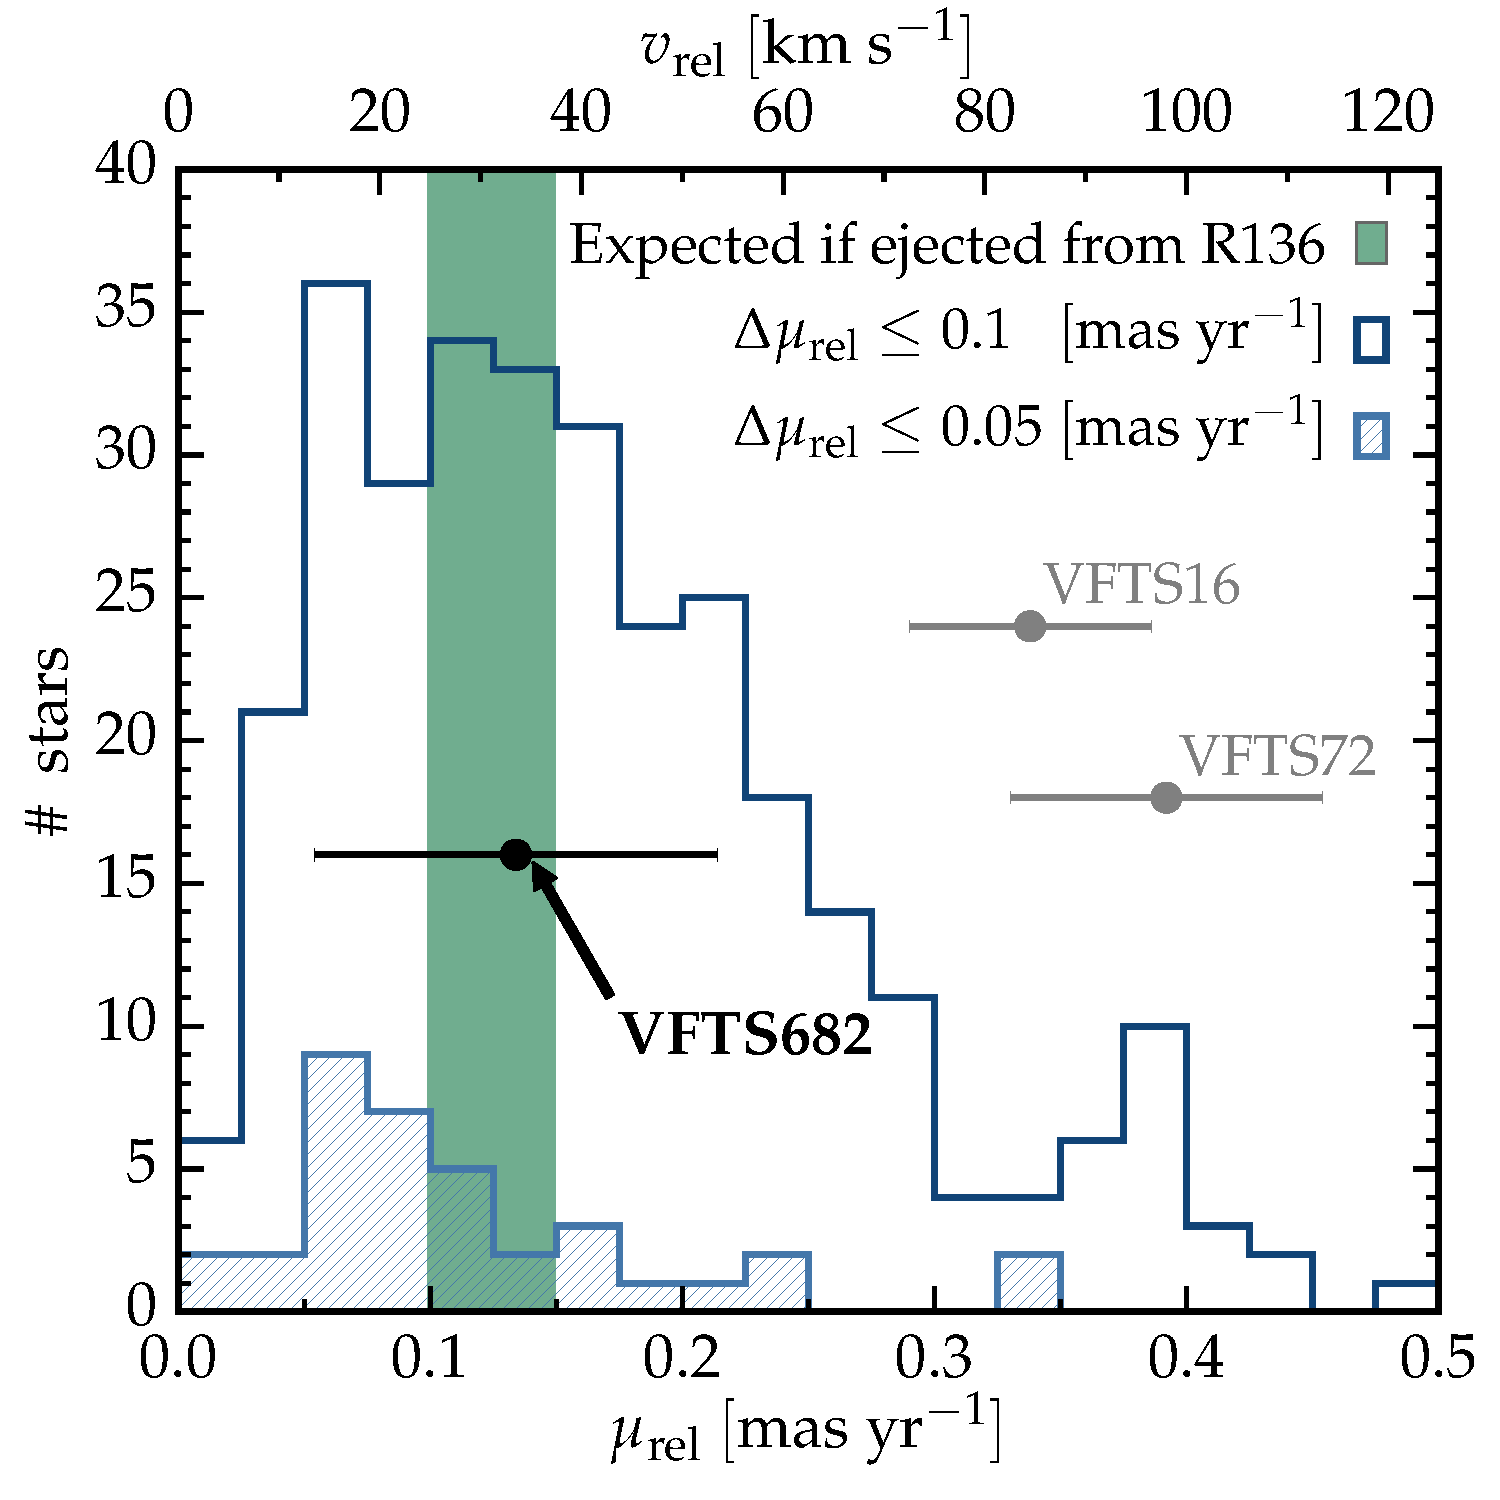
\includegraphics[width=0.35\textwidth]{figures/dist_mu_region.pdf}
  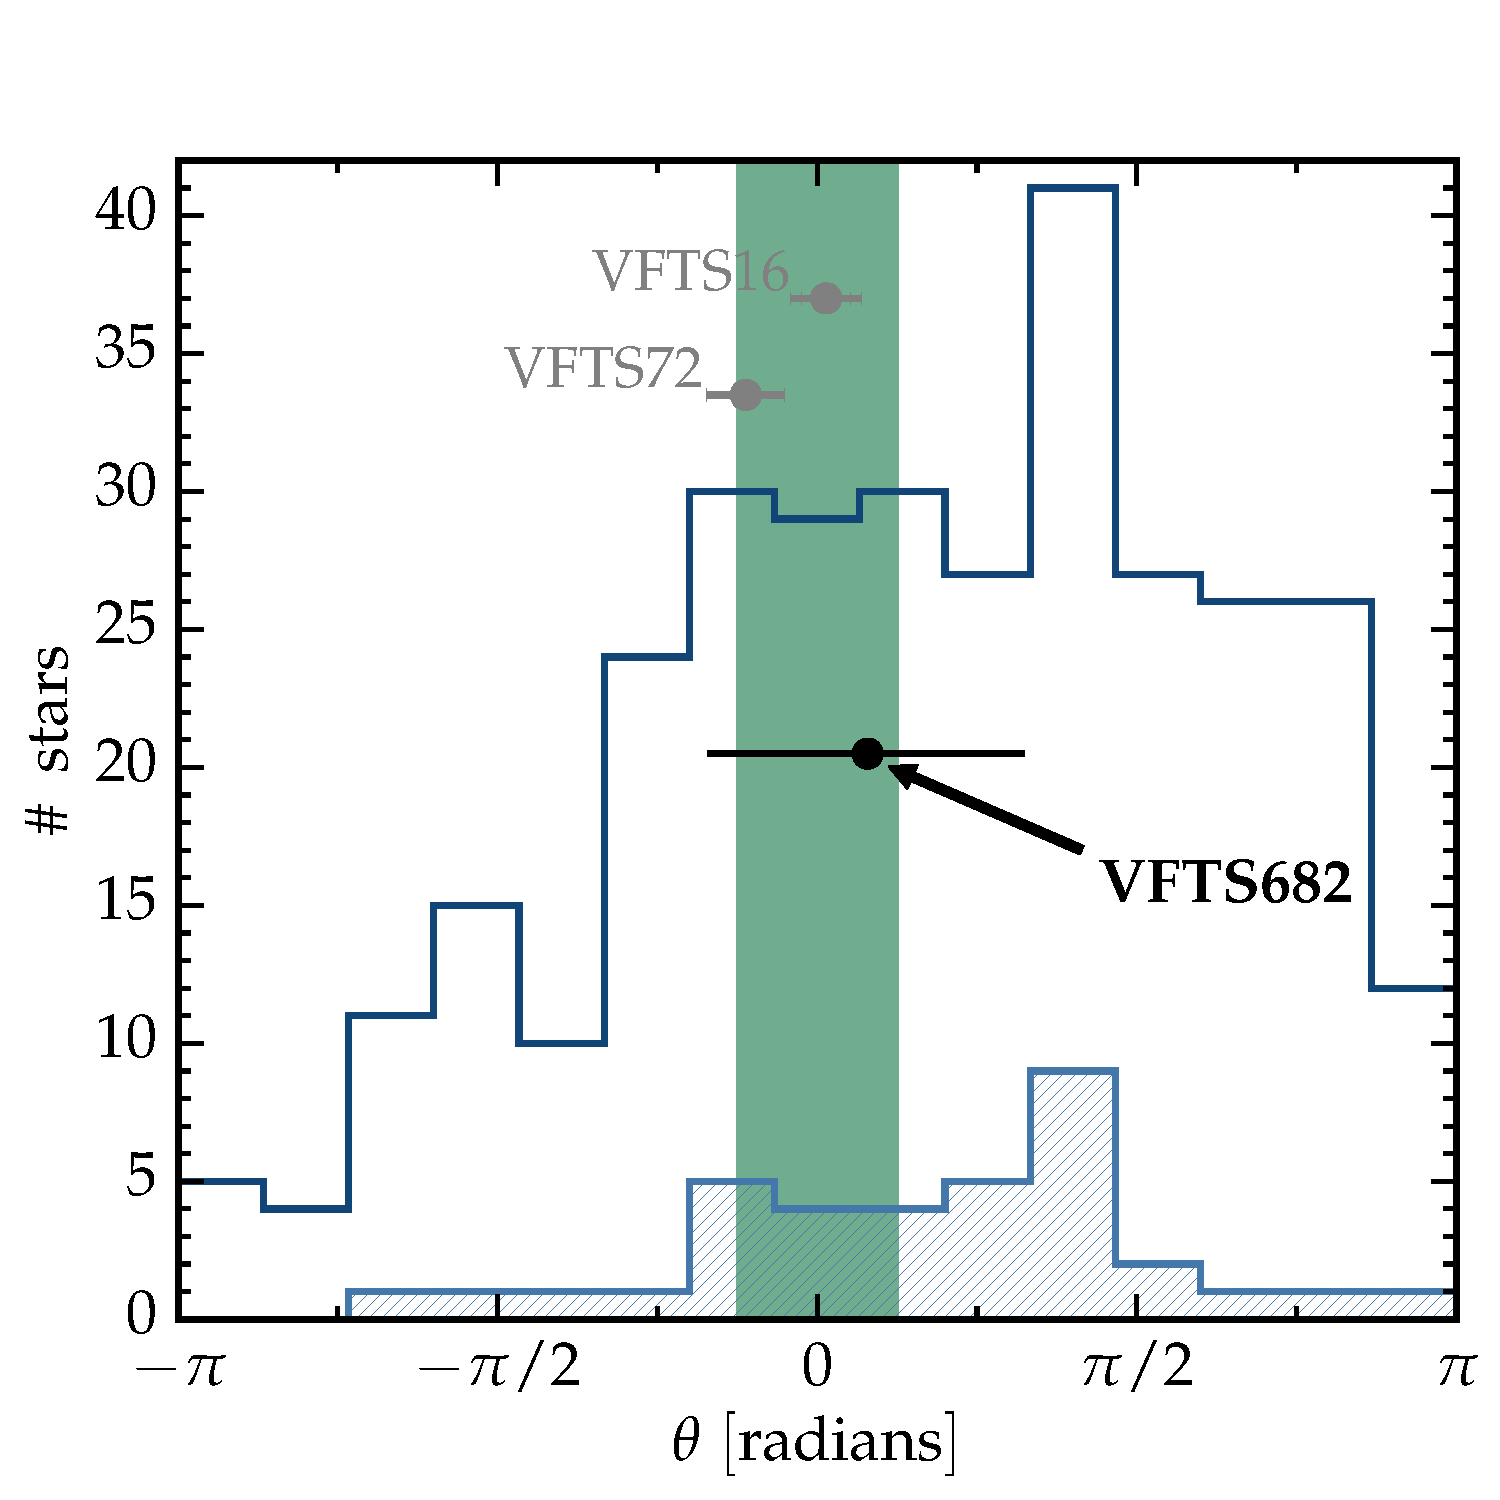
\includegraphics[width=0.35\textwidth]{figures/angle}
  \caption{\emph{Left panel}: distribution of OB-type and Wolf-Rayet stars in proper
    motion relative to R136. VFTS682 is not an outlier, but
    its relative proper motion matches the expected value if it were indeed
    ejected from R136 assuming an age of $1.0\pm0.2$\,Myr. The top axis shows the conversion to physical units
    assuming a distance of 50\,kpc. \emph{Right panel}:  distribution of
    angles between the relative proper motion direction and the radial
    direction from the center of the cluster to the star. The error bars from \emph{Gaia} for VFTS682 are large, but
    the best value is in agreement with the hypothesis of dynamical
    ejection. The peak at $\theta\simeq\pi/2$ is due to stars
    belonging to NGC2060. In both
    panels, the dark blue histograms contain 317 
    stars with error smaller than $0.1\,\mathrm{mas \
      yr^{-1}}\simeq25\,\mathrm{km\ s^{-1}}$ at 50\,kpc, the
    lighter blue histograms contain 36 stars with errors smaller than $0.05\,\mathrm{mas \
      yr^{-1}}$. }
  \label{fig:dist}
\end{figure*}

VFTS682 is identified with the source id 4657685637907503744 in the
\emph{Gaia} DR2 catalog\footnote{\url{https://vizier.u-strasbg.fr/viz-bin/VizieR-3?-source=I/345/gaia2}}
  as a 15.65 mag star in the G band
\citep{gaia:16,brown:18}.   The number of visibility periods,
i.e., groups of observations separated from other groups by a gap of at
least four days, used in the astrometric solution is seventeen for this
star. The reported astrometric excess noise is zero.  These values
suggest that the \emph{Gaia} DR2  data for VFTS682 are
reliable.

Gaia provides absolute proper motions.  To determine the relative proper motion with respect to R136, we follow  \citet{lennon:18} to define the motion of the local frame of reference using the average proper motion of nearby stars with reliable astrometric data.  They select  bright ($G<17$) stars within 0.05 degrees of R136 and exclude sources with proper motion errors greater than $0.01\masyr$ in both coordinates (see their  Sect.~2.1 for further discussion).  

With these we compute the relative proper motion
$\delta\mu_\mathrm{RA}$ and $\delta\mu_\mathrm{DEC}$.   We also compute the total projected 2d velocity
$v_\mathrm{2d}$ and
the angle $\theta$ between the direction of motion and the vector
connecting the center of R136 with the current position of VFTS 682,
i.e. such that $\theta = 0$ is the angle corresponding to perfectly
radial motion away from R136.    We further provide the projected 2d velocity
$v_\mathrm{2d}$.   All kinematic quantities are provided in
Tab.~\ref{tab:vfts682}. 



\subsection{HST astrometry for VFTS682}

The 30 Doradus region was target of an a two-epoch photometric campaign with HST providing observations in the F775W filter in October 2011 and October 2014 (GO-12499; P.I.: D.~J.~Lennon, \citealt{sabbi:13}). Visually, the star is clearly isolated and does not appear to have any close neighbor. This by itself gives further confidence in ability of \emph{Gaia} to measure the proper motion reliably without being affected by crowding. 

\citet{platais:15, platais:18} analyzed the HST data to determine the
relative proper motion and identify candidate runaway stars. The
brightest stars (V$<$14) are saturated in the data set and have been
excluded from the analysis.  VFTS682 should be one of the brightest
stars in the region, however, the high extinction makes it faint enough such that saturation effects are not an issue.   VFTS682 is relatively slow and is therefore not discussed in their paper.  However, their measurements are useful here, since they provides an  estimate of the proper motion of VFTS682 that is independent from the \emph{Gaia} measurement. 
 
The HST provides proper motions that are relative to the bulk motion of the majority of the stars in the field of view. The full 30 Dor field is covered by different pointings and there is some systematic distortion.  However, even for stars far from 30 Dor the effect is small, no more than $0.05\masyr$ across the whole 30 Dor field. The effect is much smaller for stars close to the center of field, such as VFTS 682 \citet{platais:18}.  We can therefore use the relative proper motion as a good estimate for the proper motion relative to R136. 
 
We list the relative proper motion in \Tabref{tab:vfts682}. 

\section{The kinematics of VFTS682}
\label{sec:results}

Figure~\ref{fig:dist} illustrates the kinematic properties of VFTS OB-type
and Wolf-Rayet stars in the 30 Doradus region with \emph{Gaia} DR2 errors on the proper motion
components of less than $0.1\,\mathrm{mas\ yr^{-1}}$ (dark blue lines,
including VFTS682), and less than $0.05\,\mathrm{mas\ yr^{-1}}$ (light shaded
blue). The green vertical bands show the expectations for VFTS682 if
it were ejected from R136. We highlight the star together with the two O-type
runaways \mbox{(re-)identified} by \cite{lennon:18} (VFTS16 and VFTS72,
respectively).

The left panel shows the distribution in two-dimensional proper motion relative
to R136. Although VFTS682 is not peculiar, its relative proper motion
falls in the range expected for it to reach its present day isolation
within its apparent age (green vertical band), hinting at it being a ``slow-runaway'' as
suggested by \cite{bestenlehner:11}. Subtracting
the mean motion of R136, we obtain relative proper motions (projected
velocities) of $\delta \mu_{Gaia}=0.13\pm 0.09\masyr (32\pm 21\kms)$ and
$\delta \mu_{HST}=0.20\pm 0.10\masyr (47 \pm 24\kms )$. Both values
are consistent with each other, but also with no relative motion
within $2\sigma$.

% The left panel shows the distribution in two-dimensional proper motion relative
% to R136, and shows that, although VFTS682 is not a peculiar star in terms of
% its motion relative to R136. Subtracting the mean motion of the field,
% we obtain $\delta \mu_{Gaia}=0.13\pm 0.09\masyr (32\pm 21\kms)$ and
% $\delta \mu_{HST}=0.20\pm 0.10\masyr (47 \pm 24\kms )$. Both values
% are consistent with each other and indicate
% a non-zero peculiar projected motion that would make it a slow runaway
% star as expected by \cite{bestenlehner:11} if the star was ejected
% from the cluster,  but in both cases the meaurements are also consistent with zero within 2$\sigma$. 
% More importantly, both the proper motion
% measurement from \emph{Gaia} and HST fall in the range expected to
% reach its present day location % at $\sim$29\,pc from the cluster core
% if the
% star was ejected very early in its evolution. This range is
% highlighted by the green vertical band, and its width is determined by
% the uncertainty in the present-day age of the star (cf.~\Tabref{tab:star_param}).

The right panel shows the distributions in projected flight direction for these
stars: $\theta$ is the angle between the projected radial direction from the
center of R136 to each star and its projected relative proper motion (see also \Figref{fig:main}). Dynamical ejections from the
cluster should %are expected to
produce
close to radial ejections, i.e.~$\theta\simeq0$. On this panel, the green band highlights
% the range of angles corresponding to
an opening angle around the
projected radial direction of 45\,degrees. The direction of motion of VFTS682 % is
% poorly constrained because of the large errors on the proper motion
% components both in HST and \emph{Gaia} data, but
% it
is consistent with dynamical ejection from R136. We note that
VFTS72 has a small radial velocity, while VFTS16 (and possibly VFTS682) has
large peculiar radial velocity and therefore accurate distances along
the line of sight are
needed to contrain the flight direction in three dimensions.

Figure~\ref{fig:main} shows the projected motion of VFTS682 relative to R136 on the
sky. We also show VFTS16 and VFTS72 for completeness
\citep[see][]{lennon:18}. The thick yellow arrows are proportional to
the relative proper motion from \emph{Gaia} DR2, and the thick green
line illustrates the relative proper motion from HST. The error cone
on the direction of motion is illustrated by the corresponding
prolongation in the direction opposite to the motion, and we also show
the most likely origin of the stars accounting for their apparent age.
This figure illustrates that R136 is the most likely origin of these stars, although the large error bars
prevent a robust identification for VFTS682, and there is some tension
between the apparent age and the present day distance from the cluster
core for VFTS16 and VFTS72 \citep[][]{lennon:18}. 

Assuming VFTS682 indeed originates from R136, we can calculate its kinematic
age simply as:
\begin{equation}
  \label{eq:kin_age}
  \tau_\mathrm{kin} = \frac{d_\parallel}{\delta\mu_{Gaia}} \simeq
  \frac{119.4\,\mathrm{arcsec}}{0.13\masyr} \simeq 0.9\pm\,0.6\, \mathrm{Myr} \ \ ,
\end{equation}
where $d_\parallel = 119.4\,\mathrm{arcsec}$ is the angular distance from VFTS682 to
the core of the cluster \citep[corresponding to $\sim$29\,pc at LMC distance,][]{bestenlehner:11}.
As in the rest of this study, we neglect for
simplicity the error on the distance estimates, because it is negligible compared to other uncertainties.
The kinematic age $\tau_\mathrm{kin}$ is compatible with a very early
ejection from the cluster, given the apparent age of the star.
% of $1.0\pm 0.2$\,Myr 
% \citep{schneider:18}.

Therefore, although the motion of VFTS682 is not an outlier compared
to other massive stars with small proper motion errors in \emph{Gaia} DR2, it is possible to tentatively claim that it is
a slow runaway with velocity compatible with dynamical ejection from
R136 early in the evolution of both the star and the cluster. 

% \subsection{Is it a runaway star?}
% \label{sec:runaway}
% We first address the question whether VFTS682 is a typical star
% from the kinematic point of view (which is what would be expected if it formed in relative isolation), or whether has a significant peculiar velocity compared to its surrounding population (which is what we would expect if the star has a runaway origin).  

% After subtracting the mean proper motion of the field, we obtain the relative two-dimensional relative proper motion. We obtain  $\delta \mu_{Gaia}=0.13\pm 0.09\masyr (32\pm 21\kms)$   and $\delta \mu_{HST}=0.20\pm 0.10\masyr (47 \pm 24\kms )$. 

% Both indicate a non-zero peculiar 2D motion that would make it a slow runaway star, but in both cases the meaurements are also consistent with zero within 2 sigma. 

% Figure~\ref{fig:mu_dist} shows the distribution of relative proper motions for other VFTS O, B and WR stars subselecting either those with relative proper motion errors smaller than $0.1\masyr$ (yielding 317 stars) or a more restrictive cut including only those with proper motion errors smaller than $0.05\masyr$ (yielding 36) stars.   We see that the derived Gaia proper motion is very typical for stars in the field. 

% \SdM{XXX We need to rethink }


%Therefore, two completely independent measures of the proper motion of VFTS682 relative to the surrounding field, one from HST and one from \emph{Gaia} DR2, yield values of the peculiar three-dimensional velocity of VFTS682 % (\Eqref{eq:speed_around_HST} and
% \Eqref{eq:speed_around_Gaia}, respectively)
%which would make it the most massive runaway star known to date. However, the large errors on both the proper motion measures require confirmation with future astrometric data. 

%Subtracting the mean proper motion components given by \citet{lennon:18} from the proper motion of VFTS682 (see \Tabref{tab:vfts682}), we obtain the components of proper motion of the star relative to the surrounding region $\delta\mu_\mathrm{RA}^{Gaia} = 0.10 \pm 0.07\masyr$ and $\delta\mu_\mathrm{DEC}^{Gaia} = 0.08 \pm 0.09\masyr$. These components result in a two-dimensional relative proper motion of $\delta \mu^{Gaia}=0.13\pm 0.09\,\mathrm{mas\ yr^{-1}}$.

% \begin{equation}
%   \label{eq:pm_gaia_around}
%   \delta \mu^{Gaia} = \sqrt{\left(\delta\mu_\mathrm{RA}^{Gaia}\right)^2+\left(\delta\mu_\mathrm{DEC}^{Gaia}\right)^2}
%   = 0.13\pm 0.09\,\mathrm{mas\
%   yr^{-1}} \ \ .
% \end{equation}

% Figure \Figref{fig:pm_polar} shows the distribution in relative proper motion
% of the stars used in \cite{lennon:18} to define the frame of reference
% we also adopt here, cf.~the right panel in their Fig.~2. The
% proper motions are decomposed in the radial and tangential direction
% from R136, to highlight the likelihood of it being the origin of fast
% moving stars. The plus sign marks VFTS682, which sits at the edge of
% the proper motion distribution, but is not a clear outlier. Most
% relevant is the direction of the proper motion of VFTS682, which we
% discuss in \Secref{sec:r136_origin}.



%The proper motion components can be converted into the components of the relative transverse velocity $\delta v_\mathrm{RA}^{Gaia}=24\pm19\,\kms$, $\delta v_\mathrm{DEC}^{Gaia}=20\pm23\,\kms$, assuming a distance of 50\,kpc. These can be combined obtaining a projected two-dimensional velocity of $31\pm21\kms$. 

%The radial velocity from \cite{bestenlehner:11} then gives the third component along the line of sight,  which added in quadrature to the transverse components results in a three-dimensional velocity of $44 \pm 21\kms$.
% \begin{equation}
%   \label{eq:speed_around_Gaia}
%   v_\mathrm{pec}^{Gaia} = \sqrt{\left(\delta v_\mathrm{RA}^{Gaia}\right)^2
%     +\left(\delta v_\mathrm{DEC}^{Gaia}\right)^2+\left(\delta
%       v_\mathrm{rad}^{VFTS}\right)^2} = 44 \pm 21
%   \kms \ .
% \end{equation}



% \subsection{Does it come from the R136 cluster?}
% \label{sec:r136_origin}

% Assuming that the best estimate of the peculiar velocity of VFTS682
% are reliable, we now address the question of its likely origin.

% Figure~\ref{fig:mu_dist} shows the distribution in proper motion relative to R136
% of OB-type and Wolf-Rayet stars included both in the VFTS survey and
% \emph{Gaia DR2} with reliable astrometric solutions. The bottom panel
% shows the distribution in angles $\theta$ between the relative proper motion
% direction and the direction from the core of R136 to the star. We
% emphasize that our subset of stars with reliable proper motion
% measurements is biased towards the fast moving objects, which results in a
% distribution of angles mildly peaked at small angles.

% VFTS682 is not an outlier in relative proper motion%  compared
% % to the two O-type runaways (re-)identified by \cite{lennon:18} (see
% % also below)
% . However, the star was expected to be a ``slow runaway'' by \citet{bestenlehner:11} in
% the dynamical ejection scenario. The green shade in
% \Figref{fig:mu_dist} shows the range of relative proper motions
% required to reach the present day location within
% the uncertainties on the apparent age of the star, assuming it was
% ejected from R136 very early in its life.

% Because of the large
% error bars, the angle between the relative proper motion is not very
% constraining, but it is suggestive that the best value is close to zero.
% Therefore, the relative proper motion from \emph{Gaia} DR2 are consistent with the hypothesis
% of dynamical ejection.




% \todo{discuss and find a place for Fig.2}
% The red arrow in \Figref{fig:main} shows the direction of relative proper motion of
% VFTS682 from \emph{Gaia} DR2, and the
% yellow arrows illustrate the uncertainty. % show the possible
% % range of directions within the uncertainties in the measured relative proper
% % motion.
% These arrows cross at the present-day location of VFTS682 and
% are prolonged in the direction opposite to the motion to illustrate
% the possible range of origins.
% The yellow arrow shows the direction of
% the relative proper motion from HST (see \Eqref{eq:pm_around_HST}),
% but we omit to show the possible range of directions from HST data, since it is
% insufficiently constrained to be useful.

% Although the large uncertainties on the relative proper motion
% components results in a wide range of possible directions,we argue that the most likely origin of the star is R136.

 % , which
% corroborates the idea that the star is the result of a dynamical
% ejection very soon in the cluster evolution.

% the thing below is not relevant if it is a merger, better cut out
% for now, since we are too long anyway

%Note that the
% present-day surface helium abundance
% \citep[$Y\simeq0.5$,][]{bestenlehner:11, rubio-diez:17} puts a lower
% limit on the age of the star of $\sim$0.9\,Myr, corresponding to the time needed to
% synthesize this amount of helium in the models from \cite{kohler:15}.


\begin{figure}%[tbp]
  \centering
  \includegraphics[width=0.48\textwidth]{./figures/Figure2_paper_vfts682_hst}  
  \caption{The thick yellow arrows indicate proper motions relative R136 (blue
    circle) from \emph{Gaia} DR2, multiplied by 0.4\,Myr. The prolongations in the opposite
    direction are proportional to the apparent ages of the stars, and
    the thin yellow lines illustrate the error cone on the potential
    origin. The green thick arrow
    indicates the HST proper motion of VFTS682, with the relative
    error cone and prolongation proportional to its apparent
    age.}
  
  \label{fig:main}
\end{figure}


\section{Discussion}
\label{sec:discussion}

Based on our results, we tentatively claim that VFTS682 is the most massive
(slow) runaway known to date, with a peculiar two-dimensional
projected velocity with respect to R136 of
$\sim38\kms$ (averaging the \emph{Gaia} DR2 and HST
results) but compatible with zero within $2\sigma$. Due to the large error bars, this result will need
to be revisited with future astrometric data. % to be revisited as updated
% astrometric parameters from future \emph{Gaia} data releases become
% available.
If confirmed, it means that isolated star formation is
\emph{not} required to explain the isolation of VFTS682. Its proper motion suggests that it was ejected from the cluster R136
$0.9\pm0.6$\,Myr ago. Because of the exceptionally large mass
of this star, this raises the question of which stars must populate
the core of the cluster.

Dynamical ejections due to N-body interactions typically (although, not necessarily) eject the least
massive star among those interacting \cite[e.g.,][]{banerjee:12}. This means that, just
based on the kinematic properties of VFTS682, we would expect several
stars with initial masses larger than $\sim$$150\,M_\odot$ in the
cluster R136.
This is consistent with the detection
of extremely massive stars in the core of the
cluster. % The projected rotational equatorial
% velocity\footnote{However, the determination of the rotational
%   velocity for stars showing lines in emission is complicated by the optically thick wind screening the surface of the star, and should be
%   considered with caution.} of VFTS682
% reported by \cite{schneider:18} is $v\sin(i)<200\,\kms$, which is in
% line with the average rotation rate of massive stars in the region
% \citep[][]{ramirez-agudelo:15}. This suggests that VFTS682 (i) has not
% experienced rotationally induced chemically homogeneous evolution
% \citep[][]{maeder:00,demink:09}, and (ii) it has not
% accreted mass from or merged with a binary companion, nor will it, since the multi-epoch
% data of the VFTS survey rule out the presence of a close companion at the
% present day. Moreover,

The spectral type of VFTS682
\citep[WNh5,][]{bestenlehner:11} is the same as R136a1-a3, i.e.~the
three most massive stars detected in the core of the cluster%  by
% \cite{dekoter:97,crowther:10,crowther:16}
, with an astonishing similarity in particular with
the spectrum of R136a3. Therefore, the isolation of
VFTS682 makes it an ideal target to constrain the stellar physics of
stars with masses well above $\sim$$100\,M_\odot$ while avoiding
crowding issues. %  : its isolation makes
% it an easier target for observations compared to the similar stars
% present in the crowded core of R136.

\citet{banerjee:12} used N-body simulations of fully segregated
clusters with all massive stars in binaries to suggest that VFTS682
was ejected from R136. They
demonstrated that the cluster potential does not significantly change
the velocity of the star after the ejection. In their
model, they relied on (dynamically driven) stellar mergers to explain the high masses of
VFTS682 and the massive members of R136.%  While it is not possible to
% robustly exclude that VFTS682 is itself a merger, its spectrum does not show any of the obvious signatures
% like fast rotation, which however could have already slowed down
% because of the wind angular momentum losses during and after the
% merger.

To eject such a massive object, the cluster is
expected to have produced
a large number of massive runaways. Indeed, several %relatively
isolated massive stars are observed in the region, some with known
large radial velocities and/or proper motion. % (see
% \Figref{fig:pm_polar} and Sana et al., in prep.).
A comprehensive study of the kinematic
properties of all the massive stars surrounding R136 might shed light
on whether some can be unequivocally identified as merger products. It
is also possible that the star or binary that caused the ejection of
VFTS682 might have been ejected in the opposite direction, and is also
isolated at present day. If the ejection was caused by an interaction
with a binary, however, it is likely that the binary scattered in the
opposite direction will experience further dynamical interactions on
its way, modifying its trajectory and making it difficult to find.  %absence of proof would not undermine our conclusions 

The similarities between VFTS682 and the WNh5 stars in the core of
R136 are also in agreement with the ``bully binary'' model of
\cite{fujii:11}. Based on their numerical results, they suggested that
early in the evolution of a cluster, dynamical interactions form an extremely
massive binary, which then tightens its orbit by ejecting other stars passing
by. Interpreting our results for VFTS682 through the lens of their simulations
suggests the presence of a close binary with total mass
$M_1+M_2\gtrsim 300\,M_\odot$ in the core of the cluster. Such bully
binary could be R145 according to \cite{fujii:11}, and it might be an
ideal observational candidate for a dynamically formed progenitor system of
a binary black-hole, provided that stars this massive can avoid a
pair-instability supernova \cite[e.g.,][]{rakavy:67} at LMC
metallicity \citep[see also][]{langer:07}. Similarly, the final fate of VFTS682 could be either a
pair-instability supernova without compact remnant formation, or
possibly direct collapse to a black hole above the $2^\mathrm{nd}$
mass gap. The amount of mass loss of these stars will determine their final core
mass and thus their final fate.

The kinematic age of VFTS682 puts an
upper limit to the timescale to form the ``bully binary'' in
R136. The cluster must have been at the very beginning of its
evolution, given the age estimate of $\lesssim 2$\,Myr
\citep[][]{crowther:10,sabbi:12} and the kinematic age of VFTS682. If the
cluster is indeed younger than the shortest stellar lifetime
\citep[$\sim$3\,Myr, e.g.,][]{brott:11, zapartas:17}, then the alternative
explanation for ejection of VFTS682 from the disruption of a binary
by a core-collapse event is excluded since the region is too young for stars
to have experienced core-collapse already.

The variability of VFTS682, reminiscent of LBV stars, suggests
that VFTS682 (and therefore its analogs in the core of R136) might
experience enhanced mass loss episodes in LBV eruptions. \citet{smith:15} made the highly
debated\footnote{See, e.g., \cite{humphreys:16, davidson:16, smith:16}.}
claim that LBV stars are typically isolated from O-type stars. The fact that VFTS682 is a dynamically
ejected runaway which might evolve into an LBV star suggests that
N-body interactions also play a role in explaining the apparent
isolation of at least some LBV stars. 


\citet{lennon:18} carried out a study similar to ours on the fast
moving O-type stars
in the region, and found two very massive runaway stars in the 30 Doradus region. One of them (VFTS 16)
was previously known as a runaway star from its line of sight velocity
\citep[][]{evans:10}. \citet{lennon:18} also concluded that VFTS16 is 
the result of a dynamical ejection from the R136 cluster, while the
origin of the other star (VFTS 72) is less clear given its direction
of motion (cf.~\Figref{fig:dist}). The value of $\tau_\mathrm{kin}\simeq0.9$\,Myr we find for
VFTS682 is smaller than the
corresponding value for VFTS16: \cite{lennon:18} inferred a kinematic
age of $\sim$1.5\,Myr, possibly in tension with the apparent age of that star. This means that the more
massive VFTS682 was ejected later than VFTS16 from the same cluster.

The numerical simulations from \cite{oh:16} suggest that dynamical
interaction eject the majority of the stars during or shortly after the cluster
core-collapse. The large number of isolated massive stars around it
suggest that R136 has already evolved past the
time of maximum stellar density. This might have implications for the
question of whether the cluster formed via a monolithic collapse, or
as a (potentially ongoing) merger of several sub-structures \citep[e.g.,][]{sabbi:12}.

\citet{oh:16} also showed that the mass and velocity distribution of the ejected star depends on the cluster initial conditions
(whether it is segregated, its primordial binary fraction and initial period
distribution of the binary population), therefore studies on
the population of isolated massive stars in the surroundings of R136
might shed light on its initial stellar population and dynamical
state. 

VFTS682 is potentially the most massive runaway known to date, and its ejection
from the cluster R136 likely implies that it is only the ``tip of the
iceberg'' of possibly extremely massive runaways in the
region. Studies of this population, enabled by recent HST and \emph{Gaia} observations will put constraints on the evolution
of these extreme stars, together with the formation and evolution of
the central cluster itself.



 \bibliographystyle{apj}
 \bibliography{bibliography/vfts682,my_bib}

\section*{Affiliations}
\noindent $^{1}${Astronomical Institute Anton Pannekoek, University of
    Amsterdam, 1098 XH Amsterdam, The Netherlands} \\
  $^{2}$ {ESA, European Space Astronomy Centre, Apdo. de Correos 78,
    E-28691 Villanueva de la Ca\~nada, Madrid, Spain} \\
 $^{3}$ {
 %Center for Astrophysical Sciences, 
 Department of Physics \& Astronomy, Johns Hopkins University, Baltimore, MD 21218, USA}\\
  $^{4}$ {Space Telescope Science Institute, 3700 San Martin Drive,
    Baltimore, MD 21218, USA}\\
  $^{5}${Department of Physics and Astronomy, Hicks Building,
    Hounsfield Road, University of Sheffield, Sheffield S3 7RH, UK}\\
  $^{6}${UK Astronomy Technology Centre, Royal Observatory Edinburgh, Blackford Hill, Edinburgh, EH9 3HJ, UK}\\
  $^{7}$ {National Research Council, Herzberg Astronomy \&
    Astrophysics, 5071 West Saanich Road, Victoria, BC, V9E 2E7,
    Canada}\\
  $^{8}$ {School of Astronomy \& Space Science, University of the Chinese
    Academy of Sciences, Beijing 100012, China}\\
  $^{9}$ {National Astronomical Observatories, Chinese Academy of
    Sciences, Beijing 100012, China}\\
  $^{10}$ {Argelander-Instit\"ut f\"ur Astronomie, Universit\"at Bonn,
    Auf dem H\"ugel 71, 53121, Bonn, Germany}\\
  $^{11}$ {Centro de Astrobiología, CSIC-INTA, Carretera de Torrejón a Ajalvir km-4, E-28850 Torrejón de Ardoz, Madrid, Spain}\\
  $^{12}$ {Institute of Astronomy, KU Leuven, Celestijnenlaan 200 D, B-3001 Leuven, Belgium}\\
  $^{13}$ {Department of Physics, University of Oxford, Keble Road,
    Oxford OX1 3RH, UK} \\
  $^{14}$ {Armagh Observatory, College Hill, Armagh BT61 9DG, UK}\\

  

 \begin{acknowledgements}
   \small
   We are grateful to J.~Heyl, M.\,C.\,Ramirez-Tannus, S.~N.~Shore, and S.\,Torres
   % and C.\,J.\,Evans
   for help and discussions, European Unions Horizon 2020 research and innovation programme from the European Research Council (ERC), Grant agreement No. 715063 [SdM], the NRC-Canada Plaskett Fellowship [VHB].
   
This work has made use of data from the European Space Agency (ESA) mission {\it Gaia} (\url{https://www.cosmos.esa.int/gaia}), processed by the {\it Gaia} Data Processing and Analysis Consortium (DPAC, \url{https://www.cosmos.esa.int/web/gaia/dpac/consortium}). Funding for the DPAC has been provided by national institutions, in particular the institutions
participating in the {\it Gaia} Multilateral Agreement. 
\end{acknowledgements}




\end{document}
%%% Local Variables:
%%% mode: latex
%%% TeX-master: t
%%% End:
